\documentclass[11pt,a4paper]{report}

\usepackage[T1]{fontenc}
\usepackage{lmodern}

\usepackage[a4paper,margin=2.5cm]{geometry}
\usepackage{graphicx}
\usepackage{booktabs}
\usepackage{longtable}
\usepackage{array}
\usepackage{tabularx}
\usepackage{listings}
\usepackage{xcolor}
\usepackage{tikz}
\usetikzlibrary{positioning}
\usepackage{microtype}
\usepackage{enumitem}
\usepackage{fancyhdr}
\usepackage{titlesec}
\usepackage[hidelinks]{hyperref}

\hbadness=10000

\lstdefinestyle{cppstyle}{
  language=C++,
  basicstyle=\ttfamily\small,
  keywordstyle=\color{blue},
  stringstyle=\color{teal},
  commentstyle=\color{gray},
  numbers=left,
  numberstyle=\tiny,
  stepnumber=1,
  numbersep=8pt,
  breaklines=true,
  frame=single,
  columns=fullflexible
}

\setlength{\parindent}{0pt}
\setlength{\parskip}{6pt}
\linespread{1.05}
\setlist{itemsep=3pt, topsep=4pt, parsep=0pt}

\titleformat{\chapter}
  {\bfseries\Large}
  {Chapter \thechapter ---}
  {0.6em}
  {}
\titlespacing*{\chapter}{0pt}{-6pt}{12pt}

\titleformat{\section}
  {\bfseries\normalsize}
  {\thesection}
  {0.6em}
  {}
\titlespacing*{\section}{0pt}{10pt}{6pt}

\pagestyle{fancy}
\fancyhf{}
\fancyhead[L]{Pinacoteca}
\fancyhead[R]{\nouppercase{\leftmark}}
\fancyfoot[C]{\thepage}
\renewcommand{\headrulewidth}{0.4pt}
\renewcommand{\footrulewidth}{0pt}
\setlength{\headheight}{14pt}
\addtolength{\topmargin}{-2pt}

\title{Pinacoteca\\Project Documentation}
\author{Elettro5.B}
\date{\today}

\begin{document}
\hypersetup{pageanchor=false}
\maketitle
\thispagestyle{empty}
\pagenumbering{roman}
\chapter*{Abstract}
\addcontentsline{toc}{chapter}{Abstract}
This documentation describes the Pinacoteca project in full, with a focus on software architecture, control logic, simulation, and validation. It includes requirements, traceability, design rationale, test procedures, and known limits, providing a professional and verifiable overview.
\tableofcontents
\clearpage
\pagenumbering{arabic}
\hypersetup{pageanchor=true}

\chapter{Introduction}

The \textbf{Pinacoteca} project delivers a management system for a gallery, covering access control, climate, humidity, lighting, and LCD visualization. The goal is to integrate sensors and actuators into a modular Arduino firmware, with unit tests runnable on a PC and a repeatable build flow.

This documentation is meant to describe both the technical solution and the rationale behind design choices. Each section dives into the behavior step by step, highlighting safety aspects, adopted trade-offs, and the reasoning behind the exposed APIs.

The main features are:
\begin{itemize}
  \item counting entrances and exits with a servo-assisted turnstile;
  \item indicating available capacity with a LED traffic light;
  \item temperature regulation with heating or cooling modes;
  \item humidity control with threshold and actuator (LED in simulation);
  \item ambient light control with a photoresistor and dimmer;
  \item a 16x2 LCD panel with informative pages.
\end{itemize}

The code is structured into independent modules under \texttt{lib/}. This choice reduces cross-dependencies, makes behavior easier to read, and simplifies validation through unit tests.

The system is built around reliability: if a sensor reading is invalid, control modules switch to a fallback behavior that turns outputs off, avoiding unsafe or non-deterministic states.

\chapter{Architecture}

The firmware follows a deterministic execution cycle: initialization in \texttt{setup()} and periodic module updates in \texttt{loop()}. Each module exposes \texttt{begin()} and \texttt{update()} to separate configuration from runtime logic, reducing the risk of inconsistent states.

\section{Logical layout}
\begin{itemize}
  \item \textbf{Turnstile}: reads IN/OUT buttons, updates the people count, and moves the servo.
  \item \textbf{Stoplight}: displays availability using green/red LEDs.
  \item \textbf{Thermostat}: reads the NTC sensor and decides heating/cooling.
  \item \textbf{LightingControl}: reads the photoresistor and adjusts the dimmer.
  \item \textbf{HumidifierControl}: reads the DHT22 and turns humidity control on or off.
  \item \textbf{DisplayPanel}: alternates LCD pages with status, date/time, and diagnostics.
\end{itemize}

\section{Data flow}
The flow follows three constant steps:
\begin{enumerate}
  \item \textbf{Acquisition}: analog or digital readings from sensors.
  \item \textbf{Validation}: error checks and threshold filters.
  \item \textbf{Actuation}: LED, PWM, or servo based on decisions.
\end{enumerate}
The display aggregates module states and presents a concise view for the operator.

\section{Timing cycles}
Some modules use internal timing to avoid rapid transitions or flicker. In particular:
\begin{itemize}
  \item the thermostat applies a pause before switching mode;
  \item the display caps refresh at 1 second and switches page every 5 seconds.
\end{itemize}
These choices prevent oscillations and improve perceived stability.

\section{Key parameters}
Target values are configured in the main file:\newline
\texttt{20.0 C} for temperature, \texttt{65\%} for humidity, \texttt{200 lux} for lighting, \texttt{5 people} as the maximum capacity.

\chapter{Design decisions and safety}

This chapter explains the technical choices and the implemented safety measures. The goal is a robust, predictable, and easily testable firmware.

\section{Modularity and responsibility}
Splitting the code into modules under \texttt{lib/} addresses three needs: isolate sensor logic, simplify reuse, and enable focused unit tests. Each module has a single responsibility and a minimal API surface.

The separation between \texttt{begin()} and \texttt{update()} distinguishes hardware configuration from runtime behavior. This reduces side effects and makes logic observable even in tests using mocks.

\section{Sensor error handling}
For analog and digital sensors, a consistent sentinel value is used: \texttt{-999.0} for read errors. This choice makes it easy to identify errors downstream without exceptions or complex state.

Each control module validates readings before actuating. If input is invalid, the module turns outputs off (fail-safe) and returns \texttt{false}. This prevents silent error propagation.

\section{Actuator protection and stability}
In the servo module, \texttt{antiSufferingServo} prevents motion beyond mechanical limits, logging a message on Serial. This avoids stalls or motor stress.

The thermostat introduces a pause, defined by \texttt{\_pauseTime}, to avoid rapid toggling when readings oscillate near the threshold. This improves reliability and actuator lifespan.

Lighting control uses a PWM range limited to 0--255. In Wokwi simulation, the value is forced to 255 when light is needed, ensuring visual consistency and reducing ambiguity in tests.

\section{Interface and communication choices}
The LCD is updated at most once per second and rotates pages every 5 seconds. This policy protects against excessive writes, avoids flicker, and preserves readability.

The error page summarizes operational issues (humidity high/low, abnormal temperature, people count out of range) with short texts. The choice is oriented toward quick diagnostics in real environments.

\section{Testing strategy}
The test suite validates edge conditions: sensor limits, actuator limits, state transitions, and safety fallback. Each test checks both logical output and side effects on mocked I/O.

Local Arduino mocks allow tests to run on a PC, speeding up feedback and reducing hardware dependence. This makes the project more maintainable and suitable for future evolution.

\chapter{Diagrams}

\section{Block view}
The following figure summarizes the main blocks and interactions between sensors, controls, and actuators.

\begin{center}
\resizebox{\textwidth}{!}{%
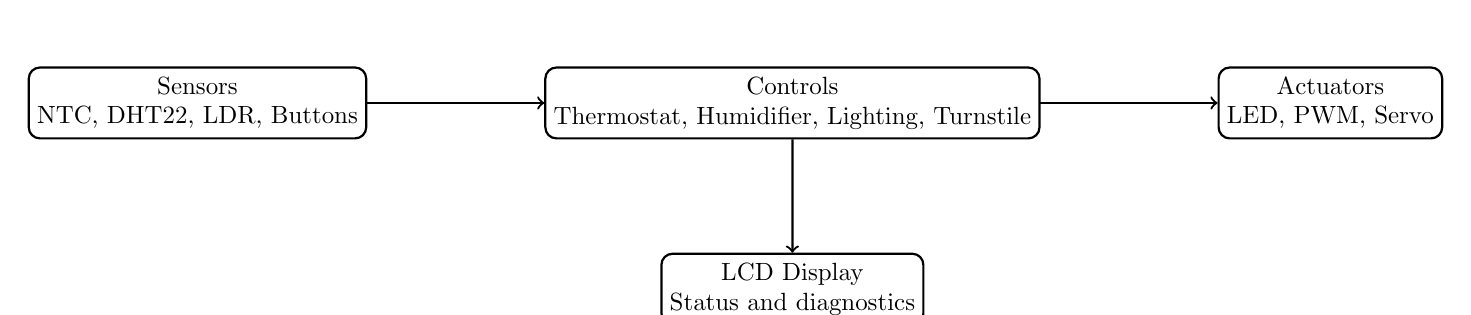
\begin{tikzpicture}[node distance=2.0cm, auto, thick, scale=0.9, transform shape]
  \tikzstyle{block} = [rectangle, draw, rounded corners, align=center, minimum width=2.4cm, minimum height=1cm]

  \node[block] (sensors) {Sensors\\NTC, DHT22, LDR, Buttons};
  \node[block, right=2.5cm of sensors] (control) {Controls\\Thermostat, Humidifier, Lighting, Turnstile};
  \node[block, right=2.5cm of control] (act) {Actuators\\LED, PWM, Servo};
  \node[block, below=1.6cm of control] (ui) {LCD Display\\Status and diagnostics};

  \draw[->] (sensors) -- (control);
  \draw[->] (control) -- (act);
  \draw[->] (control) -- (ui);
\end{tikzpicture}%
}
\end{center}

\section{Loop logical sequence}
The update cycle is designed so the display always shows the most recently computed state.

\begin{center}
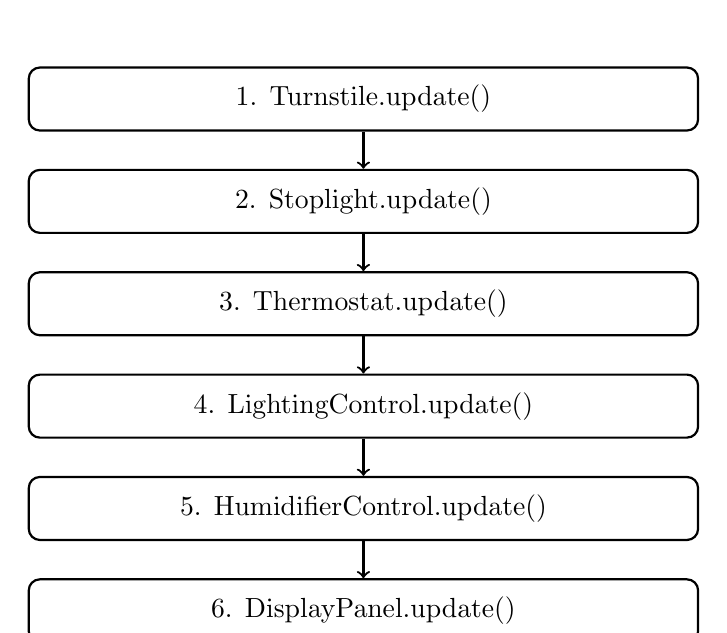
\begin{tikzpicture}[node distance=1.3cm, auto, thick]
  \tikzstyle{stepbox} = [rectangle, draw, rounded corners, align=center, minimum width=8.5cm, minimum height=0.8cm]

  \node[stepbox] (s1) {1. Turnstile.update()};
  \node[stepbox, below of=s1] (s2) {2. Stoplight.update()};
  \node[stepbox, below of=s2] (s3) {3. Thermostat.update()};
  \node[stepbox, below of=s3] (s4) {4. LightingControl.update()};
  \node[stepbox, below of=s4] (s5) {5. HumidifierControl.update()};
  \node[stepbox, below of=s5] (s6) {6. DisplayPanel.update()};

  \draw[->] (s1) -- (s2);
  \draw[->] (s2) -- (s3);
  \draw[->] (s3) -- (s4);
  \draw[->] (s4) -- (s5);
  \draw[->] (s5) -- (s6);
\end{tikzpicture}
\end{center}

\chapter{Hardware}

The Wokwi simulation described in \texttt{diagram.json} uses an Arduino Uno, a servo, buttons, LEDs, sensors, and a 16x2 LCD. The wiring matches the pins defined in the firmware, so the simulation faithfully represents the behavior expected on real hardware.

\section{Components}
\begin{itemize}
  \item Arduino Uno
  \item Servo for the turnstile
  \item 2 buttons (IN/OUT) with pull-down resistors
  \item Green and red LEDs (traffic light)
  \item Blue and orange LEDs (cooling/heating)
  \item White LED (humidity)
  \item Photoresistor (LDR)
  \item NTC sensor for temperature
  \item DHT22 sensor for humidity
  \item 4 yellow LEDs for the ceiling light (driven in parallel)
  \item 16x2 LCD
\end{itemize}

\section{Selection criteria}
Components were chosen for easy integration and the availability of stable libraries. The NTC provides a linear analog measure for the thermostat, while the DHT22 provides humidity with a simple digital interface. The 16x2 LCD balances cost and readability, with a standardized interface via \texttt{LiquidCrystal}.

\section{Pin map}
\begin{longtable}{@{}lll@{}}
\toprule
Function & Pin & Notes \\
\midrule
Turnstile servo & D3 & PWM \\
IN button & D6 & digital input \\
OUT button & D7 & digital input \\
Traffic light green LED & D4 & digital output \\
Traffic light red LED & D5 & digital output \\
Cooling LED & D8 & digital output \\
Heating LED & D9 & digital output \\
Ceiling light (PWM) & D10 & lighting dimmer \\
Humidity LED & D11 & digital output \\
Temperature sensor (NTC) & A0 & analog input \\
Photoresistor & A1 & analog input \\
LCD RS & D12 & \\
LCD EN & D13 & \\
LCD D4 & A2 & \\
LCD D5 & A3 & \\
LCD D6 & A4 & \\
LCD D7 & A5 & \\
DHT22 & D2 & pin defined in \texttt{humidity.h} \\
\bottomrule
\end{longtable}

\section{Graphical wiring schematic}
The following figure provides a compact wiring overview with Arduino at the center, sensors on the left, and actuators/display on the right. Connections are grouped by signal type (analog, digital, PWM, LCD bus) to improve readability while preserving firmware pin mapping.

\begin{center}
\resizebox{\textwidth}{!}{%
\begin{tikzpicture}[>=latex, thick, node distance=1.2cm]
  \tikzstyle{arduino}=[draw, rounded corners, minimum width=4.2cm, minimum height=8.5cm, align=center, fill=gray!14]
  \tikzstyle{sensor}=[draw, rounded corners, minimum width=3.2cm, minimum height=0.9cm, align=center, fill=green!12]
  \tikzstyle{actor}=[draw, rounded corners, minimum width=3.5cm, minimum height=0.9cm, align=center, fill=blue!12]
  \tikzstyle{groupbox}=[draw, rounded corners, dashed, line width=0.8pt, fill=gray!3]

  \draw[red!70!black, line width=1.8pt] (-8.2,4.55) -- (8.2,4.55) node[right, black, font=\scriptsize\bfseries] {+5V rail};
  \draw[black!70, line width=1.8pt] (-8.2,-4.55) -- (8.2,-4.55) node[right, black, font=\scriptsize\bfseries] {GND rail};

  \node[arduino] (uno) at (0,0) {Arduino UNO\\\small Pinacoteca firmware};

  \node[draw, fill=green!22, minimum width=0.42cm, minimum height=6.6cm, anchor=east] (hdrL) at ($(uno.west)+(0,0)$) {};
  \node[draw, fill=blue!22, minimum width=0.42cm, minimum height=6.6cm, anchor=west] (hdrR) at ($(uno.east)+(0,0)$) {};
  \node[rotate=90, font=\scriptsize\bfseries] at (hdrL.center) {INPUT HEADER};
  \node[rotate=90, font=\scriptsize\bfseries] at (hdrR.center) {OUTPUT HEADER};

  \node[groupbox, minimum width=3.8cm, minimum height=4.8cm, anchor=center] (sensorsbox) at (-6,0.6) {};
  \node[above left=0.0cm and -0.1cm of sensorsbox.north west, font=\footnotesize\bfseries] {Sensors / Inputs};

  \node[groupbox, minimum width=4.1cm, minimum height=7.5cm, anchor=center] (actorsbox) at (6,0.1) {};
  \node[above left=0.0cm and -0.1cm of actorsbox.north west, font=\footnotesize\bfseries] {Actuators / Display};

  \node[sensor] (ntc) at (-6,3.0) {Temperature NTC (A0)};
  \node[sensor] (ldr) at (-6,1.7) {Photoresistor LDR (A1)};
  \node[sensor] (dht) at (-6,0.4) {Humidity DHT22 (D2)};
  \node[sensor] (btnin) at (-6,-1.2) {IN button (D6)};
  \node[sensor] (btnout) at (-6,-2.5) {OUT button (D7)};

  \node[actor] (servo) at (6,3.2) {Turnstile servo (D3)};
  \node[actor] (tl) at (6,2.0) {Traffic LEDs green/red (D4,D5)};
  \node[actor] (clima) at (6,0.8) {Climate LEDs cool/heat (D8,D9)};
  \node[actor] (light) at (6,-0.4) {Ceiling PWM lighting (D10)};
  \node[actor] (humled) at (6,-1.6) {Humidity LED (D11)};
  \node[actor] (lcd) at (6,-3.1) {LCD 16x2 (D12,D13,A2,A3,A4,A5)};

  \node[font=\scriptsize\bfseries, text=green!50!black] at (-6,4.05) {INPUT SIDE};
  \node[font=\scriptsize\bfseries, text=blue!50!black] at (6,4.05) {OUTPUT SIDE};

  \draw[->, teal!80!black, line width=1.2pt] (ntc.east) -- node[above,sloped]{A0} ($(uno.west)+(0,2.8)$);
  \draw[->, teal!80!black, line width=1.2pt] (ldr.east) -- node[above,sloped]{A1} ($(uno.west)+(0,1.8)$);
  \draw[->, purple!75!black, line width=1.2pt] (dht.east) -- node[above,sloped]{D2} ($(uno.west)+(0,0.8)$);
  \draw[->, purple!75!black, line width=1.2pt] (btnin.east) -- node[below,sloped]{D6} ($(uno.west)+(0,-1.3)$);
  \draw[->, purple!75!black, line width=1.2pt] (btnout.east) -- node[below,sloped]{D7} ($(uno.west)+(0,-2.3)$);

  \draw[->, orange!90!black, line width=1.2pt] ($(uno.east)+(0,3.0)$) -- node[above,sloped]{D3 PWM} (servo.west);
  \draw[->, purple!75!black, line width=1.2pt] ($(uno.east)+(0,2.1)$) -- node[above,sloped]{D4,D5} (tl.west);
  \draw[->, purple!75!black, line width=1.2pt] ($(uno.east)+(0,1.1)$) -- node[above,sloped]{D8,D9} (clima.west);
  \draw[->, orange!90!black, line width=1.2pt] ($(uno.east)+(0,-0.2)$) -- node[above,sloped]{D10 PWM} (light.west);
  \draw[->, purple!75!black, line width=1.2pt] ($(uno.east)+(0,-1.3)$) -- node[above,sloped]{D11} (humled.west);
  \draw[->, blue!75!black, line width=1.2pt] ($(uno.east)+(0,-2.6)$) -- node[below,sloped]{LCD bus D12,D13,A2-A5} (lcd.west);

  \fill[white, draw=black] ($(uno.west)+(0,2.8)$) circle (0.07);
  \fill[white, draw=black] ($(uno.west)+(0,1.8)$) circle (0.07);
  \fill[white, draw=black] ($(uno.west)+(0,0.8)$) circle (0.07);
  \fill[white, draw=black] ($(uno.west)+(0,-1.3)$) circle (0.07);
  \fill[white, draw=black] ($(uno.west)+(0,-2.3)$) circle (0.07);
  \fill[white, draw=black] ($(uno.east)+(0,3.0)$) circle (0.07);
  \fill[white, draw=black] ($(uno.east)+(0,2.1)$) circle (0.07);
  \fill[white, draw=black] ($(uno.east)+(0,1.1)$) circle (0.07);
  \fill[white, draw=black] ($(uno.east)+(0,-0.2)$) circle (0.07);
  \fill[white, draw=black] ($(uno.east)+(0,-1.3)$) circle (0.07);
  \fill[white, draw=black] ($(uno.east)+(0,-2.6)$) circle (0.07);

  \node[draw, rounded corners, fill=white, align=left, font=\footnotesize, anchor=north west] (legend) at (-8.3,-4.5) {
    \textbf{Legend}\\
    \textcolor{teal!80!black}{\rule{0.8cm}{1.5pt}}\ Analog inputs\\
    \textcolor{purple!75!black}{\rule{0.8cm}{1.5pt}}\ Digital I/O\\
    \textcolor{orange!90!black}{\rule{0.8cm}{1.5pt}}\ PWM outputs\\
    \textcolor{blue!75!black}{\rule{0.8cm}{1.5pt}}\ LCD parallel bus
  };
\end{tikzpicture}%
}
\end{center}

\section{Wiring notes}
\begin{itemize}
  \item LEDs are connected with 220\,\textohm resistors to limit current.
  \item Buttons use 10\,k\textohm pull-down resistors to avoid floating readings.
  \item The DHT22 uses digital pin 2 and requires 5V power.
  \item The ceiling light is driven in PWM on D10, which simplifies intensity control.
\end{itemize}

\chapter{Firmware}

The main file \texttt{Pinacoteca.ino} instantiates modules and defines pins. The logic is organized in two distinct phases, providing a predictable and easily verifiable execution cycle.

\section{Setup}
During \texttt{setup()} the following are initialized:
\begin{itemize}
  \item serial for debug and diagnostics;
  \item servo and turnstile with a known initial position;
  \item traffic light, thermostat, lighting, and humidity;
  \item LCD panel with a startup message.
\end{itemize}
Initializing the servo before other modules reduces the risk of unintended movement during pin configuration.

\section{Loop}
In the main loop, each module updates its state in a coherent sequence:
\begin{enumerate}
  \item update turnstile and people count;
  \item update traffic light based on the limit;
  \item adjust climate (heating or cooling);
  \item adjust lighting;
  \item control humidity;
  \item refresh the display with current data.
\end{enumerate}
The order is intentional: human inputs are handled first, then status indicators are updated, and finally the LCD interface is refreshed. This way the display reflects the latest decision of the cycle.

\section{Error handling}
Modules that read sensors validate measurement correctness. If input is invalid, outputs are set to a safe state and the update function returns \texttt{false}. This behavior aligns with the project fail-safe philosophy.

\section{Target configuration}
Targets are passed to module constructors:
\begin{itemize}
  \item \texttt{Thermostat}: desired temperature in Celsius.
  \item \texttt{LightingControl}: target illuminance in lux.
  \item \texttt{HumidifierControl}: target humidity in percent.
  \item \texttt{Turnstile}: maximum number of people.
\end{itemize}
Centralized configuration in the main file allows quick tuning without modifying individual modules.

\chapter{Software modules}

This section describes in detail the modules in \texttt{lib/}. Each module is designed with a minimal interface and explicit internal logic, easing reuse and verification through tests.

\section{LED}
\paragraph{Purpose} The \texttt{led.h} file provides actuation primitives to write to digital or PWM pins. Centralizing these functions avoids duplication across control modules.

\paragraph{Flow} \texttt{led(pin, state)} performs a single \texttt{digitalWrite} and returns \texttt{true}. \texttt{ledDimming(pin, pwm)} performs \texttt{analogWrite} with the same scheme. A uniform return semantics simplifies tests.

\paragraph{Safety} The functions do not implement safety logic, but are used in a context where calling modules validate their inputs. This prevents a sensor error from being turned into an active actuator.

\paragraph{Choices} Keeping functions simple and stateless reduces complexity and improves behavioral predictability in tests with mocks.

\section{Servomotor and turnstile}
\paragraph{Purpose} The \texttt{servomotor.h} module protects the servo via \texttt{antiSufferingServo}.\linebreak
The \texttt{turnstile.h} module manages entrances and exits, maintaining a people counter.

\paragraph{Flow} In \texttt{Turnstile::begin}, button pins are configured and the servo is attached. In \texttt{update()}, IN/OUT buttons are read, capacity constraints are applied, and the servo is moved for opening and closing.

\paragraph{Safety} \texttt{antiSufferingServo} prevents exceeding the 0--180 range, logs a message on Serial, and returns \texttt{false}. This reduces the risk of mechanical damage. The counter prevents entries above the maximum or exits below zero.

\paragraph{Choices} An internal counter avoids external dependencies and makes the module self-contained. Checking limits before moving the servo is a safety choice that avoids unnecessary actuation.

\section{Stoplight}
\paragraph{Purpose} \texttt{stoplight.h} translates capacity state into immediate visual signals.

\paragraph{Flow} \texttt{begin()} configures pins as outputs. \texttt{update(currentPeople, maxPeople)} decides whether to turn on green or red based on the comparison.

\paragraph{Safety} No intermediate modes are provided: in unexpected conditions, the module always keeps one of the two outputs active, avoiding ambiguity for the operator.

\paragraph{Choices} Binary logic makes behavior easy to verify and minimizes interpretation errors.

\section{Temperature and thermostat}
\paragraph{Purpose} \texttt{temperature.h} converts the NTC analog reading into Celsius. \texttt{thermostat.h} decides the climate mode based on a central threshold with tolerance.

\paragraph{Flow} The temperature reader checks extreme values and returns \texttt{-999.0} on error. The thermostat reads the temperature, determines the requested action, and activates heating or cooling.

\paragraph{Safety} If the reading is invalid, the thermostat turns both outputs off and returns \texttt{false}. In addition, a time pause between state changes prevents rapid toggling that could wear components.

\paragraph{Choices} The 1.0 C tolerance creates a neutral window that stabilizes the system. The pause is a compromise between responsiveness and stability, suitable for a real environment.

\section{Humidity and control}
\paragraph{Purpose} \texttt{humidity.h} encapsulates DHT22 usage and provides a humidity reading.\linebreak
\texttt{humidifier.h} manages the actuator based on the target.

\paragraph{Flow} The sensor is initialized with \texttt{beginHumiditySensor}. \texttt{readHumidity()} returns the current value or \texttt{-999.0} on error. The humidity control compares the reading with the target and applies a tolerance.

\paragraph{Safety} On sensor error, the output is switched off. The tolerance avoids continuous oscillations around the setpoint.

\paragraph{Choices} A single sentinel value for errors simplifies integration with the display and diagnostics.

\section{Lighting}
\paragraph{Purpose} \texttt{photoresistor.h} estimates lux from a photoresistor. \texttt{lighting\_control.h} regulates the ceiling light via PWM.

\paragraph{Flow} The analog reading is converted to lux using a simplified model. The control calculates the difference from the target and decides whether to activate PWM.

\paragraph{Safety} Out-of-range readings are handled with minimum or maximum values, avoiding divisions by zero. PWM is always limited to the 0--255 range.

\paragraph{Choices} In Wokwi simulation the PWM is set to 255 when light is needed, providing clear and predictable visual behavior during tests.

\chapter{LCD Display}

The 16x2 display uses an abstraction layer defined in \texttt{display.h} (class \texttt{DisplayInterface}) and application logic in \texttt{lcd.h} (class \texttt{DisplayPanel}). This separation allows logic to be tested without directly depending on hardware.

\section{Pages}
The panel rotates three pages every 5 seconds:
\begin{itemize}
  \item \textbf{Date/Time}: calculated from \texttt{\_\_DATE\_\_}, \texttt{\_\_TIME\_\_}, and \texttt{millis()}.
  \item \textbf{Status}: temperature, humidity, and people count.
  \item \textbf{Diagnostics}: error messages or anomalies.
\end{itemize}
The error page shows critical conditions with priority, enabling quick intervention.

\section{Date and time computation}
Since there is no RTC, time is computed by combining the build timestamp with the increment of \texttt{millis()}. The base is set in the constructor, offering a coherent initial date and continuous time progression.

\section{Update}
Refresh is limited to 1 second to avoid flicker. Each update reads values from \texttt{Thermostat}, \texttt{HumidifierControl}, and \texttt{LightingControl}. The page switches every 5 seconds to allow time to read each set of information.

\section{Safety and robustness}
If a sensor value is invalid, the display shows \texttt{ERR} or an explicit message. This avoids misinterpretation and makes faults evident.

\chapter{Step-by-step implementation}

This chapter describes the operational flow for each feature, with code fragments and detailed explanations.

\section{Global initialization}
In the main file, modules are instantiated with key parameters and centrally defined pins. This choice makes the configuration easy to read.

\begin{lstlisting}[style=cppstyle]
const int PIN_SERVOMOTOR = 3;
const int PIN_GREEN_LIGHT = 4;
const int PIN_RED_LIGHT = 5;

Turnstile entranceTurnstile(PIN_IN_BUTTON, PIN_OUT_BUTTON, 5);
Stoplight trafficLight(PIN_GREEN_LIGHT, PIN_RED_LIGHT);
Thermostat mainThermostat(PIN_TEMPERATURE_SENSOR, 20.0, PIN_YELLOW_LIGHT, PIN_BLU_LIGHT);
LightingControl galleryLighting(PIN_PHOTORESISTOR, PIN_PLAFONIERE, 200);
HumidifierControl galleryHumidifier(IS_HUMIDIFIER_LED, 65.0);
DisplayPanel galleryDisplay(PIN_LCD_RS, PIN_LCD_EN, PIN_LCD_D4, PIN_LCD_D5, PIN_LCD_D6, PIN_LCD_D7, 5);
\end{lstlisting}

\paragraph{Rationale} Targets and capacity are centralized to reduce errors and enable quick calibration.

\section{Turnstile and people counting}
The turnstile reads buttons and moves the servo with mechanical protection.

\begin{lstlisting}[style=cppstyle]
if (inState == HIGH && _currentPeople < _maxPeople) {
    moveServo(90);
    _currentPeople++;
    delay(1000);
    moveServo(-90);
}
\end{lstlisting}

\paragraph{Steps} 1) read inputs, 2) check capacity, 3) open servo, 4) update counter, 5) close servo.

\paragraph{Safety} The counter prevents entries beyond the limit and \texttt{antiSufferingServo} prevents out-of-range movement.

\section{Capacity stoplight}
The stoplight translates the count into an immediately readable state.

\begin{lstlisting}[style=cppstyle]
if (currentPeople < maxPeople) {
    led(_greenPin, HIGH);
    led(_redPin, LOW);
} else {
    led(_greenPin, LOW);
    led(_redPin, HIGH);
}
\end{lstlisting}

\paragraph{Rationale} Two states reduce ambiguity for the operator.

\section{Thermostat}
The thermostat reads temperature and decides the action with tolerance and an anti-toggle pause.

\begin{lstlisting}[style=cppstyle]
if (temperature_celsius < (_desiredTemperature - tolerance)) {
    desired_action = 1;
} else if (temperature_celsius > (_desiredTemperature + tolerance)) {
    desired_action = 2;
} else {
    desired_action = 0;
}
\end{lstlisting}

\paragraph{Steps} 1) read sensor, 2) validate, 3) compare with target, 4) choose action, 5) actuate with pause.

\paragraph{Safety} On invalid reading, both outputs are turned off and the method returns \texttt{false}.

\section{Humidity control}
The module compares the DHT22 reading with the target and a fixed tolerance.

\begin{lstlisting}[style=cppstyle]
if (currentHumidity > (_targetHumidity + tolerance)) {
    led(_humidifierPin, HIGH);
} else if (currentHumidity < (_targetHumidity - tolerance)) {
    led(_humidifierPin, LOW);
} else {
    led(_humidifierPin, LOW);
}
\end{lstlisting}

\paragraph{Safety} If the sensor returns \texttt{NAN}, the reading becomes \texttt{-999.0} and the module turns the output off.

\section{Lighting}
Lighting control uses a simple model to translate the analog reading into lux and decide PWM.

\begin{lstlisting}[style=cppstyle]
float missingLight = _targetLux - currentLux;
if (missingLight > 0) {
    pwm_value = 255;
} else {
    pwm_value = 0;
}
ledDimming(_dimmerPin, pwm_value);
\end{lstlisting}

\paragraph{Rationale} In Wokwi simulation a full PWM is used when light is needed, making the response evident.

\section{LCD display}
The display rotates pages with different information and shows errors with priority.

\begin{lstlisting}[style=cppstyle]
if (now - _lastPageChange >= 5000) {
    _page = (_page + 1) % 3;
    _lastPageChange = now;
}
\end{lstlisting}

\paragraph{Steps} 1) limit refresh, 2) rotate page, 3) read values from modules, 4) print selected page.

\paragraph{Safety} Invalid readings are shown as \texttt{ERR} or error messages, preventing misinterpretation.

\chapter{Requirements and traceability}

This section lists the main functional requirements and their traceability to unit tests. The goal is to demonstrate that design choices are verified systematically.

\section{Functional requirements}
\begin{itemize}
  \item \textbf{R1} The system must count entrances and exits with a configurable maximum limit.
  \item \textbf{R2} The system must signal capacity status with a green/red traffic light.
  \item \textbf{R3} The system must control temperature with heating and cooling modes.
  \item \textbf{R4} The system must control humidity with threshold and tolerance.
  \item \textbf{R5} The system must control lighting with a target in lux.
  \item \textbf{R6} The display must show date/time, status, and diagnostics.
  \item \textbf{R7} In case of sensor errors, actuators must be deactivated.
\end{itemize}

\section{Test traceability}
\begingroup
\sloppy
\hbadness=10000
\tolerance=10000
\emergencystretch=1em
\scriptsize
\setlength{\tabcolsep}{2pt}
\renewcommand{\arraystretch}{1.05}
\begin{tabularx}{\textwidth}{@{}>{\raggedright\arraybackslash}p{1.0cm}>{\raggedright\arraybackslash}X>{\raggedright\arraybackslash}X@{}}
\toprule
Req. & Description & Related tests \\
\midrule
R1 & People counting with limits & \begin{tabular}[t]{@{}l@{}}\texttt{TurnstileIncrementsAndDecrementsPeople}\\\texttt{TurnstileRespectsMaxPeople}\end{tabular} \\
R2 & Capacity stoplight & \begin{tabular}[t]{@{}l@{}}\texttt{StoplightBelowMaxSetsGreen}\\\texttt{StoplightAtMaxSetsRed}\end{tabular} \\
R3 & Climate with heating/cooling & \begin{tabular}[t]{@{}l@{}}\texttt{ThermostatHeatingBranch}\\\texttt{ThermostatCoolingBranch}\end{tabular} \\
R4 & Humidity control & \begin{tabular}[t]{@{}l@{}}\texttt{HumidifierHighHumidityTurnsOnPin}\\\texttt{HumidifierLowHumidityTurnsOffPin}\end{tabular} \\
R5 & Lighting control & \begin{tabular}[t]{@{}l@{}}\texttt{LightingControlWritesPwm}\end{tabular} \\
R6 & Display pages & \begin{tabular}[t]{@{}l@{}}\texttt{DisplayPanelRotatesPages}\\\texttt{DisplayDatePageHasValidWeekdayPrefix}\end{tabular} \\
R7 & Fail-safe on sensor errors & \begin{tabular}[t]{@{}l@{}}\texttt{ThermostatSensorErrorTurnsEverythingOff}\\\texttt{HumidifierSensorErrorReturnsFalse}\end{tabular} \\
\bottomrule
\end{tabularx}
\renewcommand{\arraystretch}{1.0}
\setlength{\tabcolsep}{6pt}
\normalsize
\endgroup

\section{Notes}
Tests are executed with Arduino mocks, so checks focus on side effects (pins and LCD buffer) rather than real hardware. This approach ensures speed and repeatability.

\chapter{Tests}

The test suite uses GoogleTest and is configured in the \texttt{test/} folder. The goal is to ensure each module reacts correctly to nominal cases and edge cases, with particular attention to safety conditions.

\section{Structure}
The \texttt{CMakeLists.txt} file in \texttt{test/} downloads GoogleTest via FetchContent.
The generated executable is called \texttt{pinacoteca\_tests} and Arduino API mocks are in \texttt{test/mocks/}.
The test entry point is \texttt{all\_tests.cpp}, where each feature group has dedicated tests.

\section{Execution}
Two modes are available:
\begin{itemize}
  \item Direct CMake usage:
  \begin{lstlisting}[style=cppstyle]
cd test
cmake -S . -B build
cmake --build build -j
ctest --test-dir build --output-on-failure
  \end{lstlisting}
  \item \texttt{run\_tests.sh} script that manages build, clean, and Arduino compilation.
\end{itemize}

\section{Test rationale}
Below is the detailed explanation of the checks, with objectives, conditions, and expectations.

\subsection{LED}
\begin{itemize}
  \item \textbf{Objective}: ensure output primitives write to the correct pins.
  \item \textbf{Conditions}: direct calls to \texttt{led} and \texttt{ledDimming} with known values.
  \item \textbf{Expectations}: \texttt{digitalWrite} and \texttt{analogWrite} receive the requested value.
  \item \textbf{Tests}:
  \begin{tabular}[t]{@{}l@{}}
    \texttt{LedWriteDigitalState}\\
    \texttt{LedDimmingWritesPwm}
  \end{tabular}
\end{itemize}

\subsection{Stoplight}
\begin{itemize}
  \item \textbf{Objective}: validate green/red semantics based on capacity.
  \item \textbf{Conditions}: counts below and equal to the maximum.
  \item \textbf{Expectations}: green on below capacity, red on at full capacity.
  \item \textbf{Tests}:
  \begin{tabular}[t]{@{}l@{}}
    \texttt{StoplightBelowMaxSetsGreen}\\
    \texttt{StoplightAtMaxSetsRed}
  \end{tabular}
\end{itemize}

\subsection{Servomotor}
\begin{itemize}
  \item \textbf{Objective}: prevent movement beyond mechanical limits.
  \item \textbf{Conditions}: commands with valid angles and angles outside 0--180.
  \item \textbf{Expectations}: movement allowed within range, blocked and logged outside range.
  \item \textbf{Tests}:
  \begin{tabular}[t]{@{}l@{}}
    \texttt{AntiSufferingServoAllowsSafeMove}\\
    \texttt{AntiSufferingServoBlocksOutOfRange}
  \end{tabular}
\end{itemize}

\subsection{Turnstile}
\begin{itemize}
  \item \textbf{Objective}: count entrances/exits correctly and respect the maximum.
  \item \textbf{Conditions}: simulated IN/OUT button states; variable max people.
  \item \textbf{Expectations}: coherent increment and decrement, no limit overruns.
  \item \textbf{Tests}:
  \begin{tabular}[t]{@{}l@{}}
    \texttt{TurnstileIncrementsAndDecrementsPeople}\\
    \texttt{TurnstileRespectsMaxPeople}\\
    \texttt{TurnstileBeginConfiguresPins}
  \end{tabular}
\end{itemize}

\subsection{Temperature}
\begin{itemize}
  \item \textbf{Objective}: handle abnormal NTC sensor readings.
  \item \textbf{Conditions}: analog values at extremes (0 and 1023) and an intermediate value.
  \item \textbf{Expectations}: sentinel \texttt{-999.0} at extremes, finite value under normal conditions.
  \item \textbf{Tests}:
  \begin{tabular}[t]{@{}l@{}}
    \texttt{TemperatureReaderReturnsErrorAtExtremes}\\
    \texttt{TemperatureReaderReturnsFiniteForValidInput}
  \end{tabular}
\end{itemize}

\subsection{Thermostat}
\begin{itemize}
  \item \textbf{Objective}: verify heating/cooling logic and fail-safe behavior.
  \item \textbf{Conditions}: valid reading above/below target, and invalid reading.
  \item \textbf{Expectations}: correct pin activation, outputs off on sensor error.
  \item \textbf{Tests}:
  \begin{tabular}[t]{@{}l@{}}
    \texttt{ThermostatHeatingBranch}\\
    \texttt{ThermostatCoolingBranch}\\
    \texttt{ThermostatSensorErrorTurnsEverythingOff}\\
    \texttt{ThermostatBeginSetsPinModesAndSetGetTarget}
  \end{tabular}
\end{itemize}

\subsection{Humidity and HumidifierControl}
\begin{itemize}
  \item \textbf{Objective}: validate DHT22 reading and threshold logic.
  \item \textbf{Conditions}: high humidity, low humidity, and invalid reading (\texttt{NAN}).
  \item \textbf{Expectations}: actuator consistent with threshold and off on error.
  \item \textbf{Tests}:
  \begin{tabular}[t]{@{}l@{}}
    \texttt{HumidityReadAndError}\\
    \texttt{HumidifierHighHumidityTurnsOnPin}\\
    \texttt{HumidifierLowHumidityTurnsOffPin}\\
    \texttt{HumidifierSensorErrorReturnsFalse}\\
    \texttt{HumidifierSetGetTargetWorks}
  \end{tabular}
\end{itemize}

\subsection{Photoresistor and LightingControl}
\begin{itemize}
  \item \textbf{Objective}: ensure conversion and PWM align with the target.
  \item \textbf{Conditions}: analog values at extremes and intermediate values.
  \item \textbf{Expectations}: lux clamped at the edges and coherent PWM (255 with low light, 0 with high light).
  \item \textbf{Tests}:
  \begin{tabular}[t]{@{}l@{}}
    \texttt{PhotoresistorLuxEdgeCases}\\
    \texttt{LightingControlWritesPwm}\\
    \texttt{LightingControlBeginAndSetGetTarget}
  \end{tabular}
\end{itemize}

\subsection{DisplayInterface}
\begin{itemize}
  \item \textbf{Objective}: verify the abstract LCD layer.
  \item \textbf{Conditions}: calls to \texttt{begin}, \texttt{clear}, \texttt{setCursor}, \texttt{print}.
  \item \textbf{Expectations}: the mock LCD buffer contains the expected strings.
  \item \textbf{Tests}:
  \begin{tabular}[t]{@{}l@{}}
    \texttt{DisplayInterfaceBasicOperations}
  \end{tabular}
\end{itemize}

\subsection{DisplayPanel}
\begin{itemize}
  \item \textbf{Objective}: verify page rotation and diagnostic messages.
  \item \textbf{Conditions}: simulated time advancement and sensor value changes.
  \item \textbf{Expectations}: date/time page, status page, and error page shown in rotation.
  \item \textbf{Tests}:
  \begin{tabular}[t]{@{}l@{}}
    \texttt{DisplayPanelRotatesPages}\\
    \texttt{DisplayDatePageHasValidWeekdayPrefix}\\
    \texttt{DisplayStatusPageShowsTurnstileCountExactly}\\
    \texttt{DisplayErrorPageShowsHumidityHigh}\\
    \texttt{DisplayErrorPageShowsTurnstileError}
  \end{tabular}
\end{itemize}

\section{run\_tests.sh script}
Main options:
\begin{itemize}
  \item \texttt{--clean}: deletes the build folder.
  \item \texttt{--with-arduino}: compiles the sketch with arduino-cli.
  \item \texttt{--upload}: uploads the sketch to a board (requires \texttt{--port}).
  \item \texttt{--board <fqbn>}: selects the board, default \texttt{arduino:avr:uno}.
\end{itemize}

\chapter{Usage instructions}

\section{Test build}
To run unit tests:
\begin{lstlisting}[style=cppstyle]
make test
\end{lstlisting}
This command invokes the script and produces the test executable in the \texttt{test/build} folder.

To clean:
\begin{lstlisting}[style=cppstyle]
make test-clean
\end{lstlisting}
Cleaning is recommended when switching toolchains or updating dependencies.

\section{Arduino compilation}
To compile the sketch via the script:
\begin{lstlisting}[style=cppstyle]
./test/run_tests.sh --with-arduino --board arduino:avr:uno
\end{lstlisting}
This mode runs unit tests first and then compiles the sketch, reducing the risk of uploading unverified firmware.

To upload to a real board:
\begin{lstlisting}[style=cppstyle]
./test/run_tests.sh --upload --board arduino:avr:uno --port /dev/ttyACM0
\end{lstlisting}
Before uploading, verify that the serial port is correct.

\section{Wokwi simulation}
The simulation wiring is defined in \texttt{diagram.json}. Open the project in Wokwi and start the simulation to observe the overall behavior. The simulation is useful for validating the flow without physical hardware.

\chapter{Risks and failure modes}

This section identifies the main technical risks and implemented countermeasures. The goal is to demonstrate awareness of failure modes and a realistic mitigation strategy.

\section{Sensor risks}
\small
\begin{longtable}{@{}>{\raggedright\arraybackslash}p{3.6cm}>{\raggedright\arraybackslash}p{6.2cm}>{\raggedright\arraybackslash}p{5.2cm}@{}}
\toprule
Risk & Effect & Mitigation \\
\midrule
NTC disconnected or shorted & Incorrect or infinite reading & Sentinel value \texttt{-999.0}, outputs off \\
DHT22 not responding & Invalid humidity & Control disabled, error shown on LCD \\
Photoresistor saturated & Extreme lux & Values clamped (0 or 9999) to avoid division by zero \\
Noisy buttons & Incorrect counting & Capacity thresholds and increment/decrement logic \\
\bottomrule
\end{longtable}
\normalsize

\section{Actuator risks}
\small
\begin{longtable}{@{}>{\raggedright\arraybackslash}p{3.6cm}>{\raggedright\arraybackslash}p{6.2cm}>{\raggedright\arraybackslash}p{5.2cm}@{}}
\toprule
Risk & Effect & Mitigation \\
\midrule
Servo overtravel & Mechanical stress & \texttt{antiSufferingServo} blocks beyond 0--180 \\
Rapid climate toggling & Actuator wear & Time pause before switching state \\
Wrong PWM & Unstable lighting & PWM always in range 0--255 \\
\bottomrule
\end{longtable}
\normalsize

\section{Integration risks}
\begin{itemize}
  \item \textbf{Library dependencies}: mitigated with simple APIs and local mocks for tests.
  \item \textbf{State inconsistency}: mitigated with a fixed sequence in \texttt{loop()}.
  \item \textbf{Insufficient diagnostics}: mitigated with an LCD error page and Serial logs.
\end{itemize}

\chapter{Timing and performance}

This section describes key firmware timings and the motivations behind temporal choices.

\section{Update frequencies}
\begin{itemize}
  \item \textbf{Display}: refresh every 1 second, page change every 5 seconds.
  \item \textbf{Thermostat}: continuous checks with a 5-second anti-toggle pause.
  \item \textbf{Turnstile}: immediate response to buttons, with a 1-second delay to simulate passage.
\end{itemize}

\section{Motivations}
\begin{itemize}
  \item LCD refresh at 1 second avoids flicker and reduces redundant writes.
  \item The thermostat pause stabilizes behavior near the threshold.
  \item The turnstile delay avoids rapid double counting.
\end{itemize}

\section{Impact on the loop}
The module sequence is short and deterministic. The only intentional delay is in the turnstile, chosen to represent physical opening. In a future evolution, this delay can be replaced by a non-blocking \texttt{millis()}-based state machine.

\chapter{Known limits and roadmap}

\section{Current limits}
\begin{itemize}
  \item PWM lighting control in simulation uses a fixed value due to Wokwi limits.
  \item The turnstile uses a blocking 1-second delay during opening.
  \item Time is estimated without an RTC, based on \texttt{\_\_DATE\_\_} and \texttt{\_\_TIME\_\_}.
  \item No hardware/software debounce filters are implemented for buttons.
\end{itemize}

\section{Roadmap}
\begin{itemize}
  \item Introduce an RTC for accurate date/time.
  \item Real PWM control with lux feedback (PID or proportional control).
  \item Non-blocking turnstile control with a state machine.
  \item Software debounce for buttons and event logic.
  \item Expand tests with stress and timing cases.
\end{itemize}

\chapter{Requirements-design-test traceability}

This section links requirements, software components, and unit tests, focusing exclusively on programming and simulation aspects.

\section{Traceability matrix}
\begingroup
\sloppy
\hbadness=10000
\scriptsize
\setlength{\tabcolsep}{2pt}
\renewcommand{\arraystretch}{1.05}
\begin{tabularx}{\textwidth}{@{}>{\raggedright\arraybackslash}p{1.0cm}>{\raggedright\arraybackslash}X>{\raggedright\arraybackslash}X@{}}
\toprule
Req. & Software components & Tests \\
\midrule
R1 & \texttt{Turnstile}, \texttt{servomotor.h} & \texttt{TurnstileIncrementsAndDecrementsPeople}, \texttt{TurnstileRespectsMaxPeople} \\
R2 & \texttt{Stoplight}, \texttt{led.h} & \texttt{StoplightBelowMaxSetsGreen}, \texttt{StoplightAtMaxSetsRed} \\
R3 & \texttt{Thermostat}, \texttt{temperature.h} & \texttt{ThermostatHeatingBranch}, \texttt{ThermostatCoolingBranch} \\
R4 & \texttt{HumidifierControl}, \texttt{humidity.h} & \texttt{HumidityReadAndError}, \texttt{HumidifierSensorErrorReturnsFalse} \\
R5 & \texttt{LightingControl}, \texttt{photoresistor.h} & \texttt{PhotoresistorLuxEdgeCases}, \texttt{LightingControlWritesPwm} \\
R6 & \texttt{DisplayPanel}, \texttt{DisplayInterface} & \texttt{DisplayPanelRotatesPages}, \texttt{DisplayInterfaceBasicOperations} \\
R7 & All control modules & \texttt{ThermostatSensorErrorTurnsEverythingOff}, \texttt{HumidifierSensorErrorReturnsFalse} \\
\bottomrule
\end{tabularx}
\renewcommand{\arraystretch}{1.0}
\setlength{\tabcolsep}{6pt}
\normalsize
\endgroup

\section{Notes}
Traceability shows that each software requirement is covered by at least one test and that modules are independent and verifiable in isolation via mocks.

\chapter{Software validation and simulation}

This section describes how to validate firmware behavior in simulation and in a test environment, without entering electrical aspects.

\section{Validation strategy}
\begin{itemize}
  \item \textbf{Unit tests}: cover base functions and module logic.
  \item \textbf{Wokwi simulation}: end-to-end verification of the \texttt{loop()} cycle with virtual sensors and actuators.
  \item \textbf{Regression tests}: repeated suite execution after code changes.
\end{itemize}

\section{Simulation validation procedures}
\begin{enumerate}
  \item Start the simulation and verify display initialization.
  \item Press IN/OUT buttons and verify people count and stoplight.
  \item Force high/low temperatures and observe heating/cooling LEDs.
  \item Change humidity and observe control activation.
  \item Darken or illuminate the photoresistor and verify the ceiling light.
  \item Check LCD page rotation and error messages.
\end{enumerate}

\section{Software acceptance criteria}
\begin{itemize}
  \item No crashes or blocks in the \texttt{loop()} cycle.
  \item All modules respond coherently to simulated input values.
  \item Error conditions deactivate outputs and show diagnostics.
  \item The test suite completes successfully.
\end{itemize}

\chapter{Calibration and simulation limits}

This section describes software calibration aspects and simulation limits.

\section{Software calibration}
\begin{itemize}
  \item \textbf{Temperature}: the NTC calculation uses standard parameters (BETA, RL10). Real accuracy depends on the sensor and wiring, but the simulation model is stable.
  \item \textbf{Humidity}: the DHT22 in simulation returns ideal values; in a real environment an empirical calibration is recommended.
  \item \textbf{Lux}: conversion from the photoresistor is approximate; the target lux is a software reference rather than a certified measurement.
\end{itemize}

\section{Simulation limits}
\begin{itemize}
  \item PWM is simplified (full value when light is needed).
  \item Sensor response time is idealized.
  \item Some real phenomena (noise, drift, latency) are not reproduced.
\end{itemize}

\chapter{Trade-offs and design choices}

This section summarizes some evaluated alternatives and the motivations for the adopted solution, limited to software aspects.

\section{Time management}
\begin{itemize}
  \item \textbf{Choice}: use \texttt{delay} in the turnstile and \texttt{millis()} for display/thermostat.
  \item \textbf{Motivation}: simple to understand and sufficient in simulation.
  \item \textbf{Trade-off}: \texttt{delay} is blocking; an FSM would be more scalable.
\end{itemize}

\section{Sentinel values for errors}
\begin{itemize}
  \item \textbf{Choice}: \texttt{-999.0} for sensor errors.
  \item \textbf{Motivation}: easy to recognize and propagate.
  \item \textbf{Trade-off}: requires explicit checks in each module.
\end{itemize}

\section{Modular architecture}
\begin{itemize}
  \item \textbf{Choice}: independent modules with small APIs.
  \item \textbf{Motivation}: facilitates testing and maintenance.
  \item \textbf{Trade-off}: higher number of files and interfaces to maintain.
\end{itemize}

\chapter{Glossary}

\begin{longtable}{@{}p{3.5cm}p{11cm}@{}}
\toprule
Term & Meaning \\
\midrule
Fail-safe & Behavior that moves the system to a safe state on error. \\
FSM & Finite state machine used to manage events over time. \\
Lux & Unit of illuminance. \\
PWM & Pulse-width modulation used to regulate power. \\
Sentinel & Special value indicating an error or invalid state. \\
Wokwi & Online simulator for Arduino and electronic components. \\
\bottomrule
\end{longtable}

\chapter{Appendix: public APIs}

This appendix summarizes the main classes and functions exposed by the modules. APIs are designed to be minimal and easy to test, with a common \texttt{begin()} + \texttt{update()} pattern for control modules.

\section{Turnstile}
Manages people counting and servo actuation based on button inputs.
\begin{itemize}
  \item \texttt{Turnstile(int inButton, int outButton, int maxPeople)}
  \item \texttt{void begin(Servo* servo)}
  \item \texttt{void update()}
  \item \texttt{int getPeopleCount() const}
\end{itemize}

\section{Stoplight}
Translates capacity into a red/green visual signal.
\begin{itemize}
  \item \texttt{Stoplight(int greenPin, int redPin)}
  \item \texttt{void begin()}
  \item \texttt{void update(int currentPeople, int maxPeople)}
\end{itemize}

\section{Thermostat}
Controls heating and cooling with tolerance and an anti-toggle pause.
\begin{itemize}
  \item \texttt{Thermostat(int sensorPin, float desiredTemperature, int}\\
        \texttt{heatingPin, int coolingPin)}
  \item \texttt{void begin()}
  \item \texttt{bool update()}
  \item \texttt{void setTargetTemperature(float newTarget)}
  \item \texttt{float getTargetTemperature() const}
  \item \texttt{float getCurrentTemperature() const}
\end{itemize}

\section{HumidifierControl}
Controls humidity with sentinel handling in case of error.
\begin{itemize}
  \item \texttt{HumidifierControl(int humidifierPin, float targetHumidity)}
  \item \texttt{void begin()}
  \item \texttt{bool update()}
  \item \texttt{void setTargetHumidity(float newHumidityTarget)}
  \item \texttt{float getTargetHumidity() const}
  \item \texttt{float getCurrentHumidity() const}
\end{itemize}

\section{LightingControl}
Regulates lighting based on a target lux via PWM.
\begin{itemize}
  \item \texttt{LightingControl(int sensorPin, int dimmerPin, int targetLux)}
  \item \texttt{void begin()}
  \item \texttt{bool update()}
  \item \texttt{void setTargetLux(int newLuxTarget)}
  \item \texttt{int getTargetLux() const}
  \item \texttt{float getCurrentLux() const}
\end{itemize}

\section{DisplayPanel}
Manages the LCD UI with rotating pages and error messages.
\begin{itemize}
  \item \texttt{DisplayPanel(int rs, int en, int d4, int d5, int d6,}\\
        \texttt{int d7, int maxPeople)}
  \item \texttt{void begin()}
  \item \texttt{void update(int currentPeople, Thermostat\&,}\\
        \texttt{HumidifierControl\&, LightingControl\&)}
\end{itemize}

\section{Utility functions}
Reusable primitives for I/O and sensor readings.
\begin{itemize}
  \item \texttt{bool led(int pin, bool state)}
  \item \texttt{bool ledDimming(int pin, int pwm)}
  \item \texttt{float readTemperatureCelsius(int sensorPin)}
  \item \texttt{float readHumidity()}
  \item \texttt{float readLux(int light\_sensor\_pin)}
  \item \texttt{bool antiSufferingServo(int angle, Servo\& s)}
\end{itemize}

\chapter{Software and dependencies}

\section{Tools}
\begin{itemize}
  \item Arduino IDE or arduino-cli for compilation and upload.
  \item CMake >= 3.16 for tests.
  \item C++17 compiler for PC tests.
\end{itemize}
Using arduino-cli enables automation and integration with test pipelines.

\section{Libraries}
\begin{itemize}
  \item Servo (Arduino)
  \item LiquidCrystal (Arduino)
  \item DHT (for DHT22)
  \item GoogleTest (tests only)
\end{itemize}
Arduino libraries are used via standard headers, while GoogleTest is downloaded dynamically during CMake configuration.

\section{Repository}
The project is organized as:
\begin{itemize}
  \item \texttt{Pinacoteca.ino} for firmware;
  \item \texttt{lib/} for modules;
  \item \texttt{test/} for unit tests;
  \item \texttt{diagram.json} for Wokwi simulation.
\end{itemize}


\end{document}
